\documentclass[11pt, a4paper]{article}

\usepackage{amsmath, amssymb, titling}
\usepackage[margin=2.5cm]{geometry}
\usepackage[colorlinks=true, linkcolor=black, urlcolor=black, citecolor=black]{hyperref}
\usepackage{graphicx}
\usepackage{float}
\usepackage{fancyhdr, lastpage}
\usepackage{xcolor}

\renewcommand\maketitlehooka{\null\mbox{}\vfill}
\renewcommand\maketitlehookd{\vfill\null}

\title{Satellite Orbit Control \\ HW7}
\author{Almog Dobrescu\\\\ID 214254252}

\pagestyle{fancy}
\cfoot{Page \thepage\ of \pageref{LastPage}}

\begin{document}

\maketitle

\thispagestyle{empty}
\newpage
\setcounter{page}{1}

\tableofcontents
\vfil
\listoffigures
\newpage

\section{Given}
\begin{equation*}
    \begin{matrix}
        T_1=100\left[min\right] = 6\cdot10^3\left[sec\right] && T_2 = T_1 = 6\cdot10^3\left[sec\right] \\
        e_1 = 0 && e_2 = 0 \\
        a_1 = \sqrt[3]{\frac{\mu T_1^2}{4\pi^2}} = 7.1366\cdot10^3\left[km\right] && a_2 = a_1 = 7.1366\cdot10^3\left[km\right]
    \end{matrix}\\
\end{equation*}
\begin{equation*}
    \alpha=\Delta i = 0.01^\circ
\end{equation*}
In CW frame with origin at Satellite \#1 and at $t=0$:
\begin{equation*}
    \begin{matrix}
    \begin{pmatrix}
        x_2(0)=0 \\ y_2(0)=-1 \\ z_2(0)=1
    \end{pmatrix}\left[\mathrm{km}\right] &&
    \begin{pmatrix}
        \dot{x}_2(0)=0 \\ \dot{y}_2(0) =0 \\ \dot{z}_2(0)=-0.74267\cdot n
    \end{pmatrix}\displaystyle\left[\frac{\mathrm{km}}{\mathrm{sec}}\right]
    \end{matrix}
\end{equation*}

\subsection{Desired}
\begin{equation*}
    \begin{matrix}
    \begin{pmatrix}
        x_2(t_f)=0 \\ y_2(t_f)=0 \\ z_2(t_f)=0
    \end{pmatrix} &&
    \begin{pmatrix}
        \dot{x}_2(t_f)=0 \\ \dot{y}_2(t_f)=0 \\ \dot{z}_2(t_f)=0
    \end{pmatrix}
    \end{matrix}
\end{equation*}

\subsection{Limitations}
\begin{equation*}
    \begin{matrix}
        a_\text{max} = 4\cdot10^{-5}\left[\frac{\mathrm{km}}{\mathrm{sec}^2}\right] && t_f=2000\left[sec\right]
    \end{matrix}
\end{equation*}

\section{The CW equations}
\begin{equation}
    \left\{\begin{array}{l}
        \ddot{x}-2n\dot{y}-3n^2x=f_x\\
        \ddot{y}+2n\dot{x}=f_y\\
        \ddot{z}+n^2z=f_z
    \end{array}\right.
\end{equation}

\subsection{x-y}
\begin{equation}
    \vec{x}=\begin{pmatrix}
        x\\\dot{x}\\y\\\dot{y}
    \end{pmatrix}
\end{equation}
\begin{equation}
    \dot{\vec{x}}=F\vec{x}+G\vec{f}
\end{equation}
Where:
\begin{equation}
    \begin{matrix}
        F=\begin{pmatrix}
            0 & 1 & 0 & 0 \\
            3n^2 & 0 & 0 & 2n \\
            0 & 0 & 0 & 1 \\
            0 & -2n & 0 & 0
        \end{pmatrix} && G=\begin{pmatrix}
            0 & 0\\
            1 & 0\\
            0 & 0\\
            0 & 1
        \end{pmatrix} && f=\begin{pmatrix}
            f_x\\f_y
        \end{pmatrix}
    \end{matrix}
\end{equation}

\subsection{z}
\begin{equation}
    \vec{x}=\begin{pmatrix}
        z\\\dot{z}
    \end{pmatrix}
\end{equation}
\begin{equation}
    \dot{\vec{x}}=F\vec{x}+Gf
\end{equation}
Where:
\begin{equation}
    \begin{matrix}
        F=\begin{pmatrix}
            0 & 1 \\
            -n^2 & 0
        \end{pmatrix} && G=\begin{pmatrix}
            0 \\
            1
        \end{pmatrix} && f=\begin{pmatrix}
            f_z
        \end{pmatrix}
    \end{matrix}
\end{equation}

\subsection{x-y-z}
The equations of motion in state space form are therefor:
\begin{equation}
    \vec{x} = \begin{pmatrix}
        x & \dot{x} & y & \dot{y} & z & \dot{z}
    \end{pmatrix}^T
\end{equation}
\begin{equation}
    \dot{\vec{x}}=F\vec{x}+G\vec{f}
\end{equation}
Where:
\begin{equation}
    \begin{matrix}
        F=\begin{pmatrix}
            0 & 1 & 0 & 0 & 0 & 0 \\
            3n^2 & 0 & 0 & 2n & 0 & 0 \\
            0 & 0 & 0 & 1 & 0 & 0 \\
            0 & -2n & 0 & 0 & 0 & 0 \\
            0 & 0 & 0 & 0 & 0 & 1 \\
            0 & 0 & 0 & 0 & -n^2 & 0 
        \end{pmatrix} && G=\begin{pmatrix}
            0 & 0 & 0\\
            1 & 0 & 0\\
            0 & 0 & 0\\
            0 & 1 & 0\\
            0 & 0 & 0\\
            0 & 0 & 1
        \end{pmatrix} && f=\begin{pmatrix}
            f_x\\f_y\\f_z
        \end{pmatrix}
    \end{matrix}
\end{equation}

\section{Optimal Linear Time-Varying Gains}
It is needed to fulfill the end condition:
\begin{equation}
    \Psi\left(\vec{x}_{\left(t_f\right)}\right)=\underbrace{\Psi\vec{x}_f}_{\mathrm{q\ x\ n}}
\end{equation}
while minimazing the use of fuel:
\begin{equation}
    J=\frac{1}{2}\int_0^{t_f}\vec{f}^{\ T}\vec{f}dt
\end{equation}
We will use the Pontriagin optimization method:
\begin{equation}
    J=\vec{\nu}^T\Psi\vec{x}_f+\frac{1}{2}\int_0^{t_f}\vec{f}^{\ T}\vec{f}dt
\end{equation}
The Hemiltonian:
\begin{equation}
    \begin{matrix}
        \displaystyle H=\frac{1}{2}\vec{f}^{\ T}\vec{f}+\vec{\lambda}^T\left(F\vec{x}+G\vec{f}\right) && \mathrm{where} && \vec{\lambda}=\begin{pmatrix}
            \lambda_x\\\lambda_{\dot{x}}\\\lambda_y\\\lambda_{\dot{y}}
        \end{pmatrix}
    \end{matrix}
\end{equation}
The optimization criteria:
\begin{equation}
    \begin{matrix}
        \displaystyle\frac{\partial H}{\partial\vec{f}}=\vec{0} && \rightarrow && \vec{f}=-G^T\vec{\lambda}
    \end{matrix}
\end{equation}
and the Euler Lagrange equations:
\begin{equation}
    \begin{matrix}
        \displaystyle\dot{\vec{\lambda}}^{\ T}=-\frac{\partial Hh}{\partial\vec{x}}=-\vec{\lambda}^{\ T}F && \rightarrow && \dot{\vec{\lambda}}=-F^T\vec{\lambda}, &\displaystyle \vec{\lambda}_f^{\ T}=\frac{\partial J}{\partial\vec{x}_f}=\vec{\nu}^{\ T}\Psi
    \end{matrix}
\end{equation}
Since the current problem is linear with square preformance criteria, the Euler Lagrange equation becomes linear differential equations independent of the state vector. Hence:
\begin{equation}
    \begin{matrix}
        \vec{\lambda}_{\left(t\right)}=e^{-F^Tt}\vec{\lambda}_0 \\\\
        \begin{matrix}
            \downarrow & \vec{\lambda}_f
        \end{matrix} \\\\
        \vec{\lambda}_{\left(t\right)}=e^{-F^T\left(t-t_f\right)}\Psi^T\vec{\nu}
    \end{matrix}
\end{equation}
The equation of motion is therefore:
\begin{equation}
    \dot{\vec{x}}=F\vec{x}-GG^Te^{-F^T\left(t-t_f\right)}\Psi^T\vec{\nu}
\end{equation}
The solution of the equation is:
\begin{equation}
    \vec{x}_{\left(t\right)}=e^{Ft}\vec{x}_0-\int_0^t\left(e^{F\left(t-\tau\right)}GG^Te^{-F^T\tau}d\tau\right)e^{F^Tt_f}\Psi^T\vec{\nu}
\end{equation}
% where:
% \begin{equation}
%     \begin{array}{l}
%         e^{F\left(t-\tau\right)}=\begin{pmatrix}
            
%         \end{pmatrix}
%     \end{array}
% \end{equation}
and can be writen like:
\begin{equation}
    \begin{matrix}
       \displaystyle\vec{x}_{\left(t\right)}=e^{Ft}\vec{x}_0+M_{\left(t\right)}e^{F^Tt_f}\Psi^T\vec{\nu} &&\displaystyle M_{\left(t\right)}=\int_0^t\left(e^{F\left(t-\tau\right)}GG^Te^{-F^T\tau}d\tau\right)
    \end{matrix}
\end{equation}
The vector $\vec{\nu}$ can be found from the known final conditions:
\begin{equation}
    \begin{array}{c}
        \Psi\vec{x}_{\left(t_f\right)}=0=\Psi\left(e^{Ft}\vec{x}_0+M_{\left(t\right)}e^{F^Tt_f}\Psi^T\vec{\nu}\right) \\
        \Downarrow \\
        \vec{\nu}=-\left(\Psi M_{\left(t_f\right)}e^{F^Tt_f}\Psi^T\right)^{-1}\Psi e^{Ft_f}\vec{x}_0
    \end{array}
\end{equation}
\newpage

\section{The Results}
In our case (rendezvous), $\Psi=I$. 
\begin{figure}[H]
    \centering
    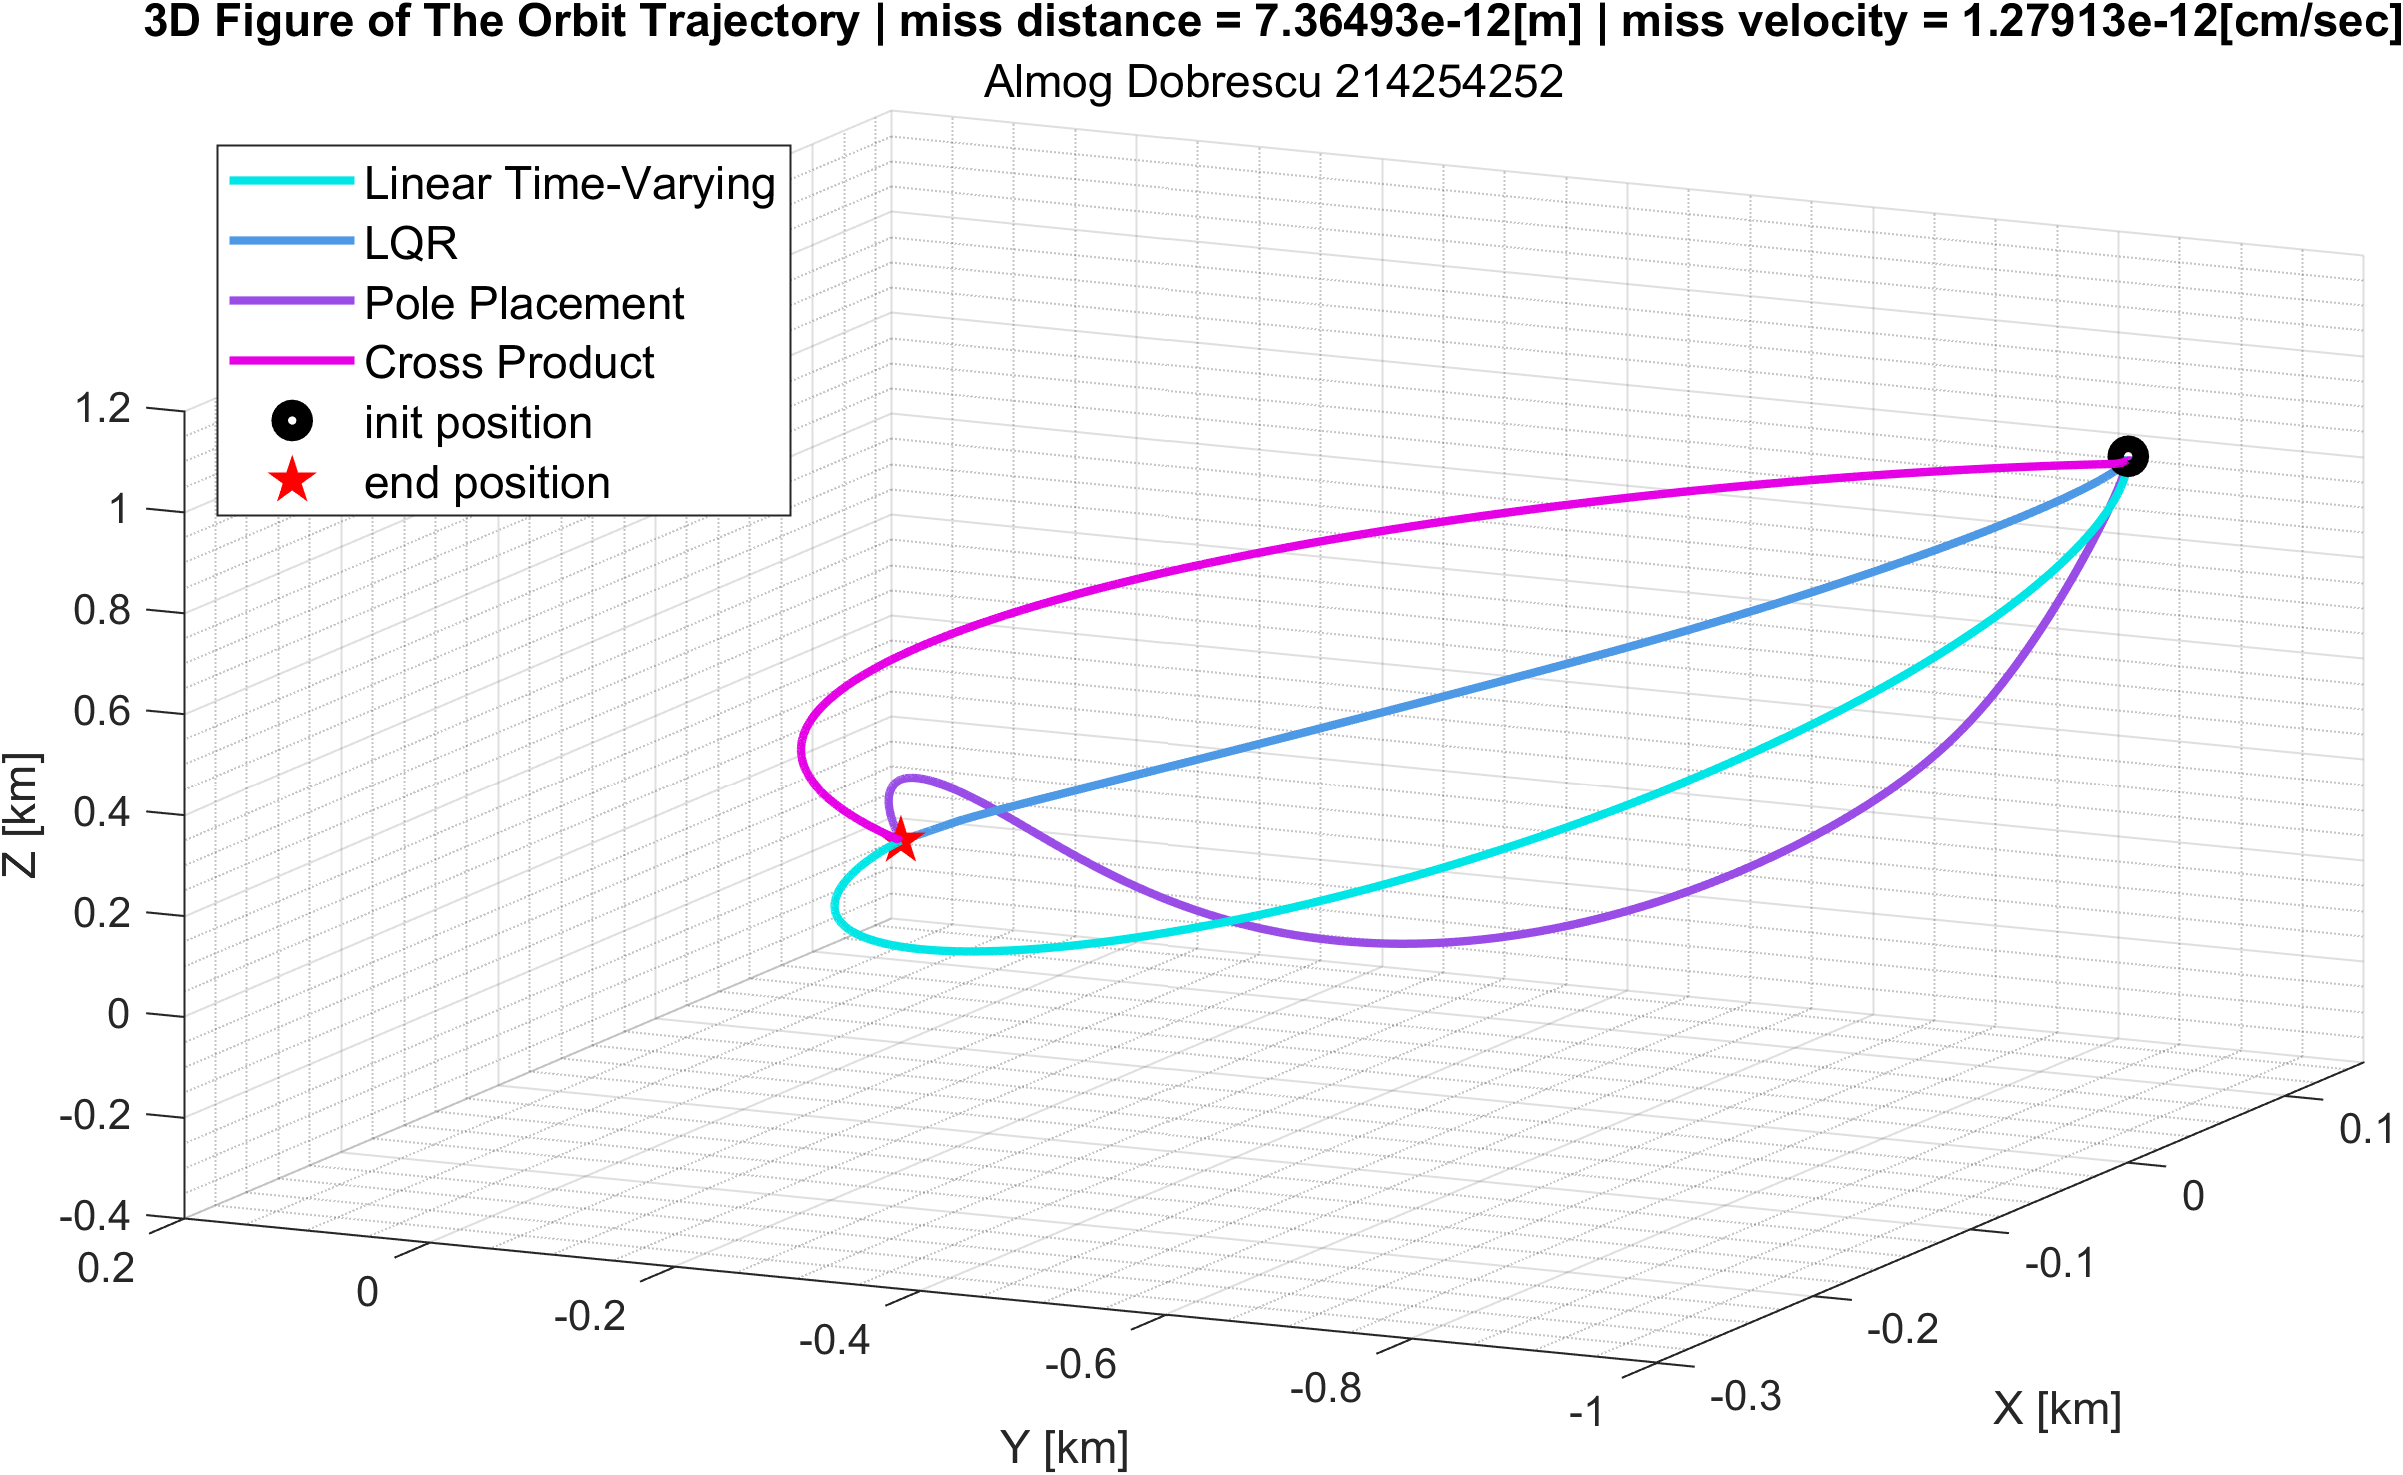
\includegraphics[width=1\textwidth]{images/graph1.png}
    \caption{3D figure of the orbit trajectory}
    \label{fig:3D-plot}
\end{figure}
\begin{figure}[H]
    \centering
    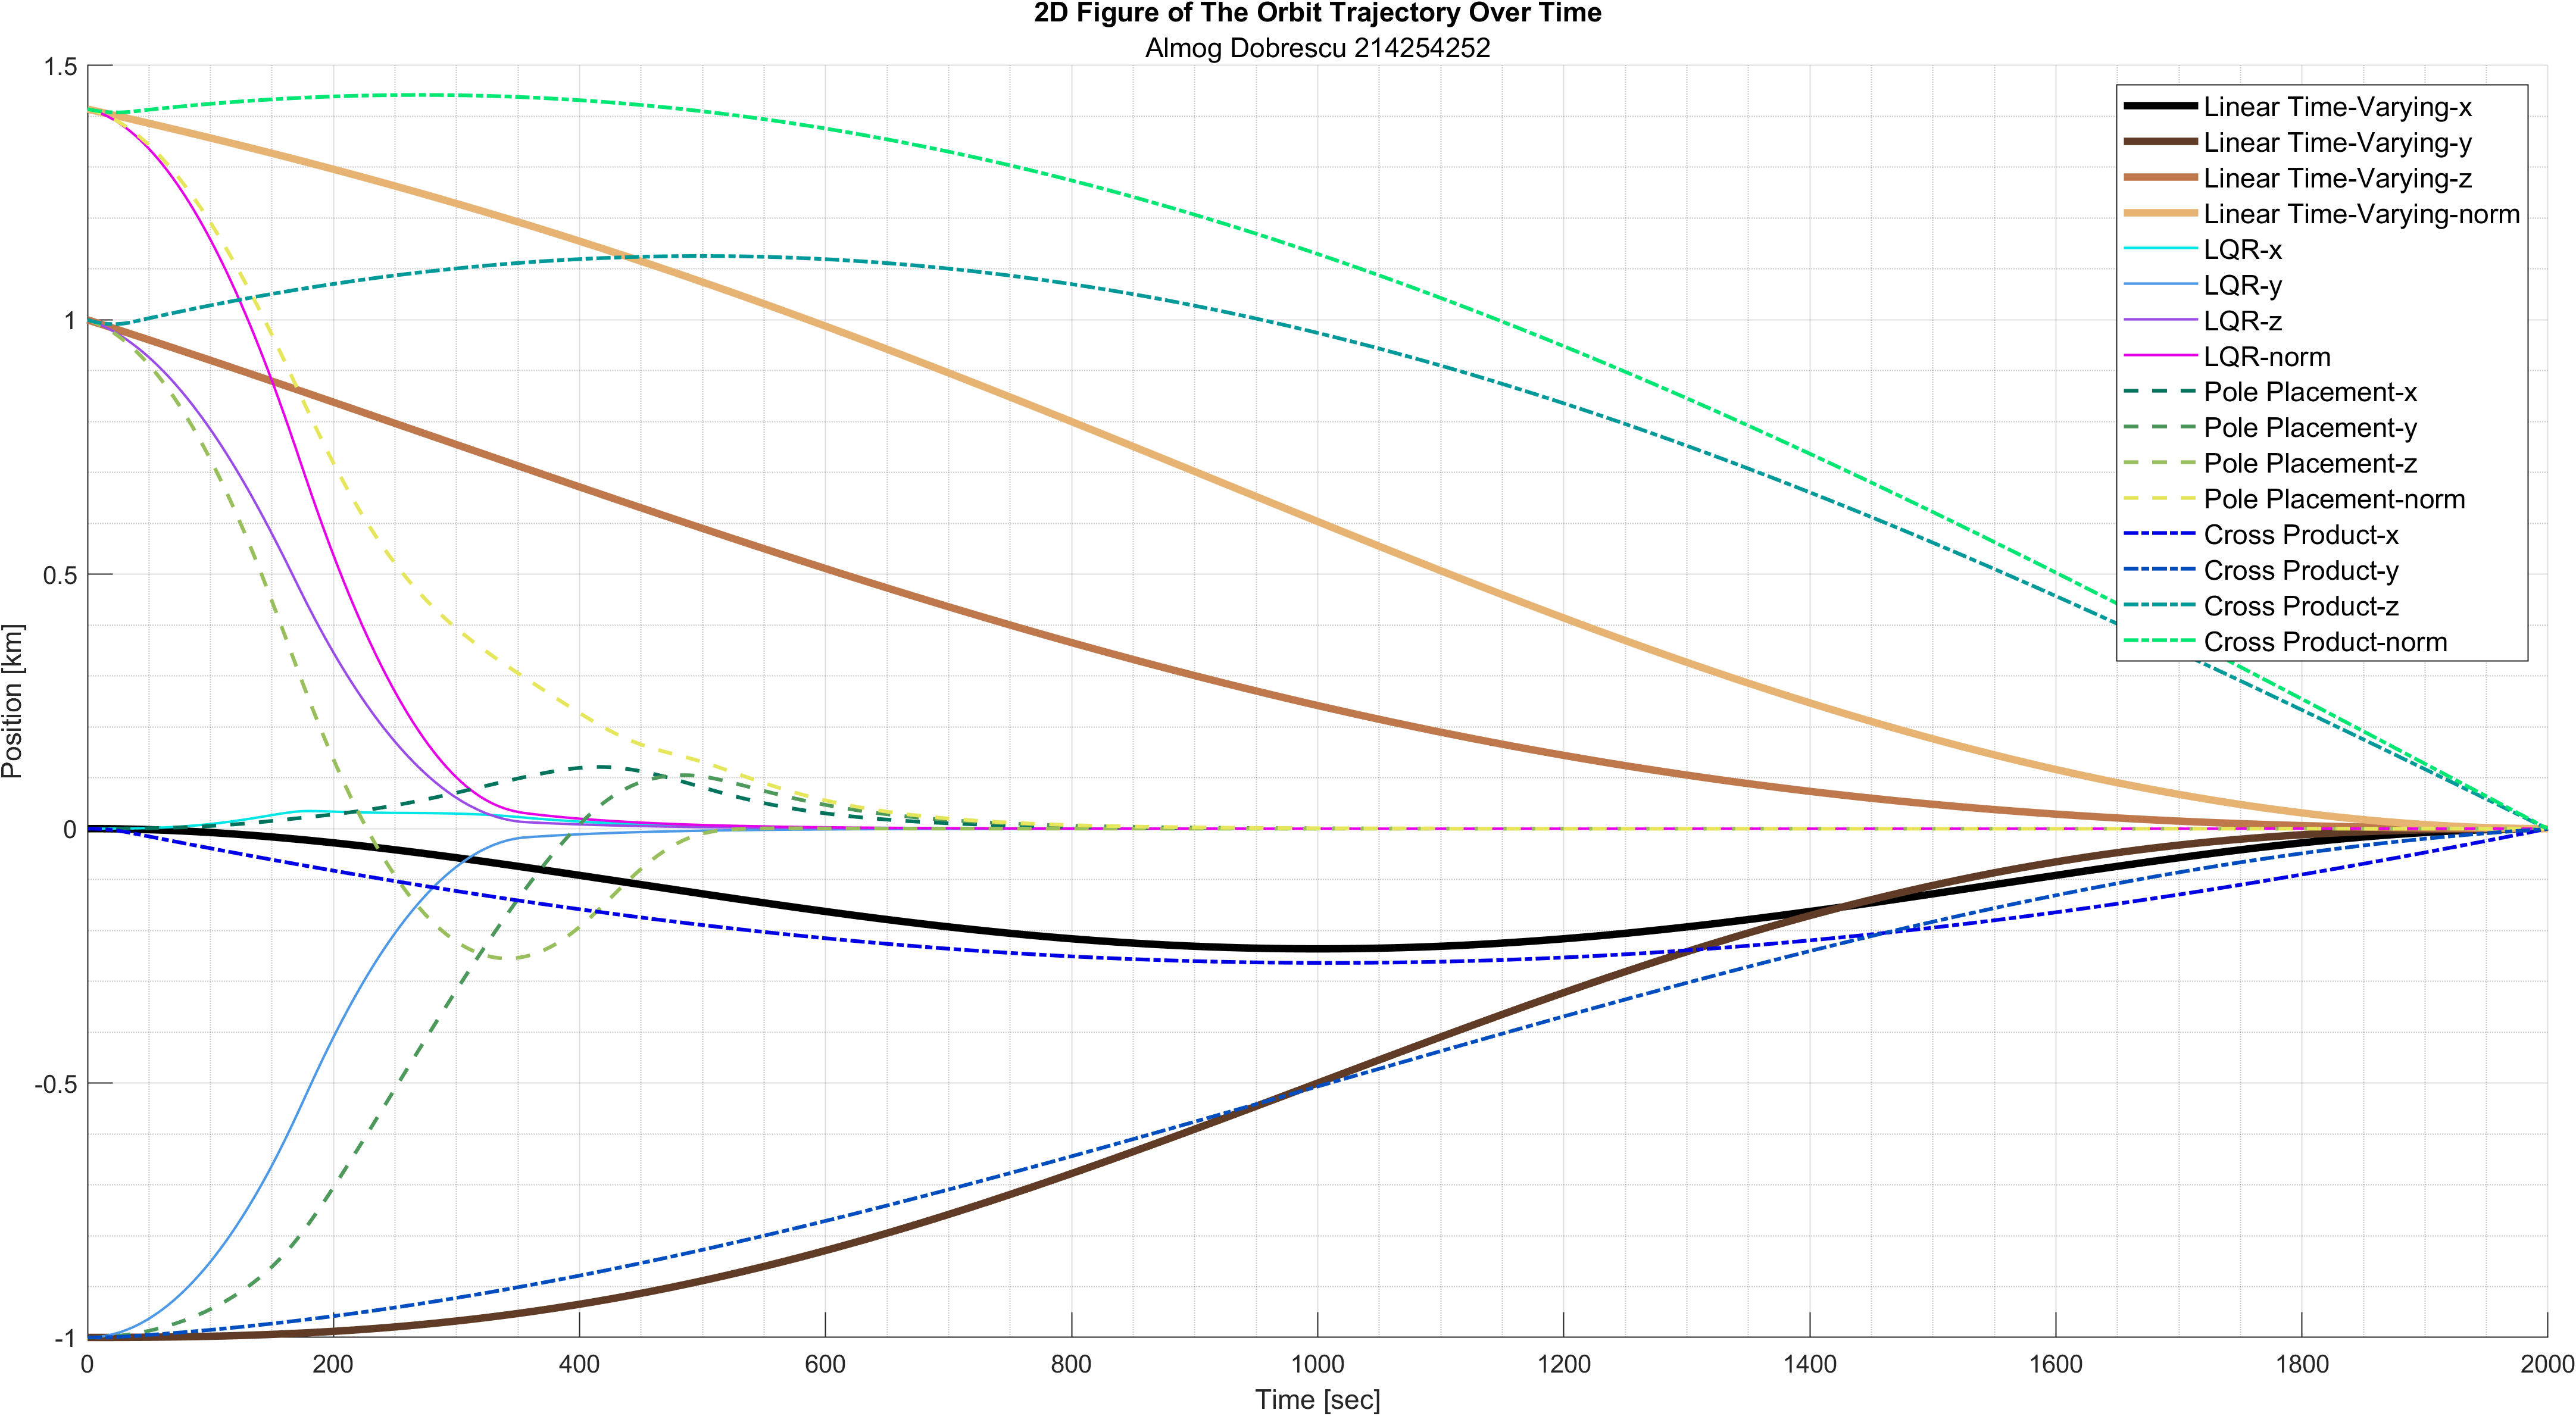
\includegraphics[width=1\textwidth]{images/graph2.png}
    \caption{2D figure of the orbit target trajectory over time}
    \label{fig:2D-plot_over_time}
\end{figure}
\begin{figure}[H]
    \centering
    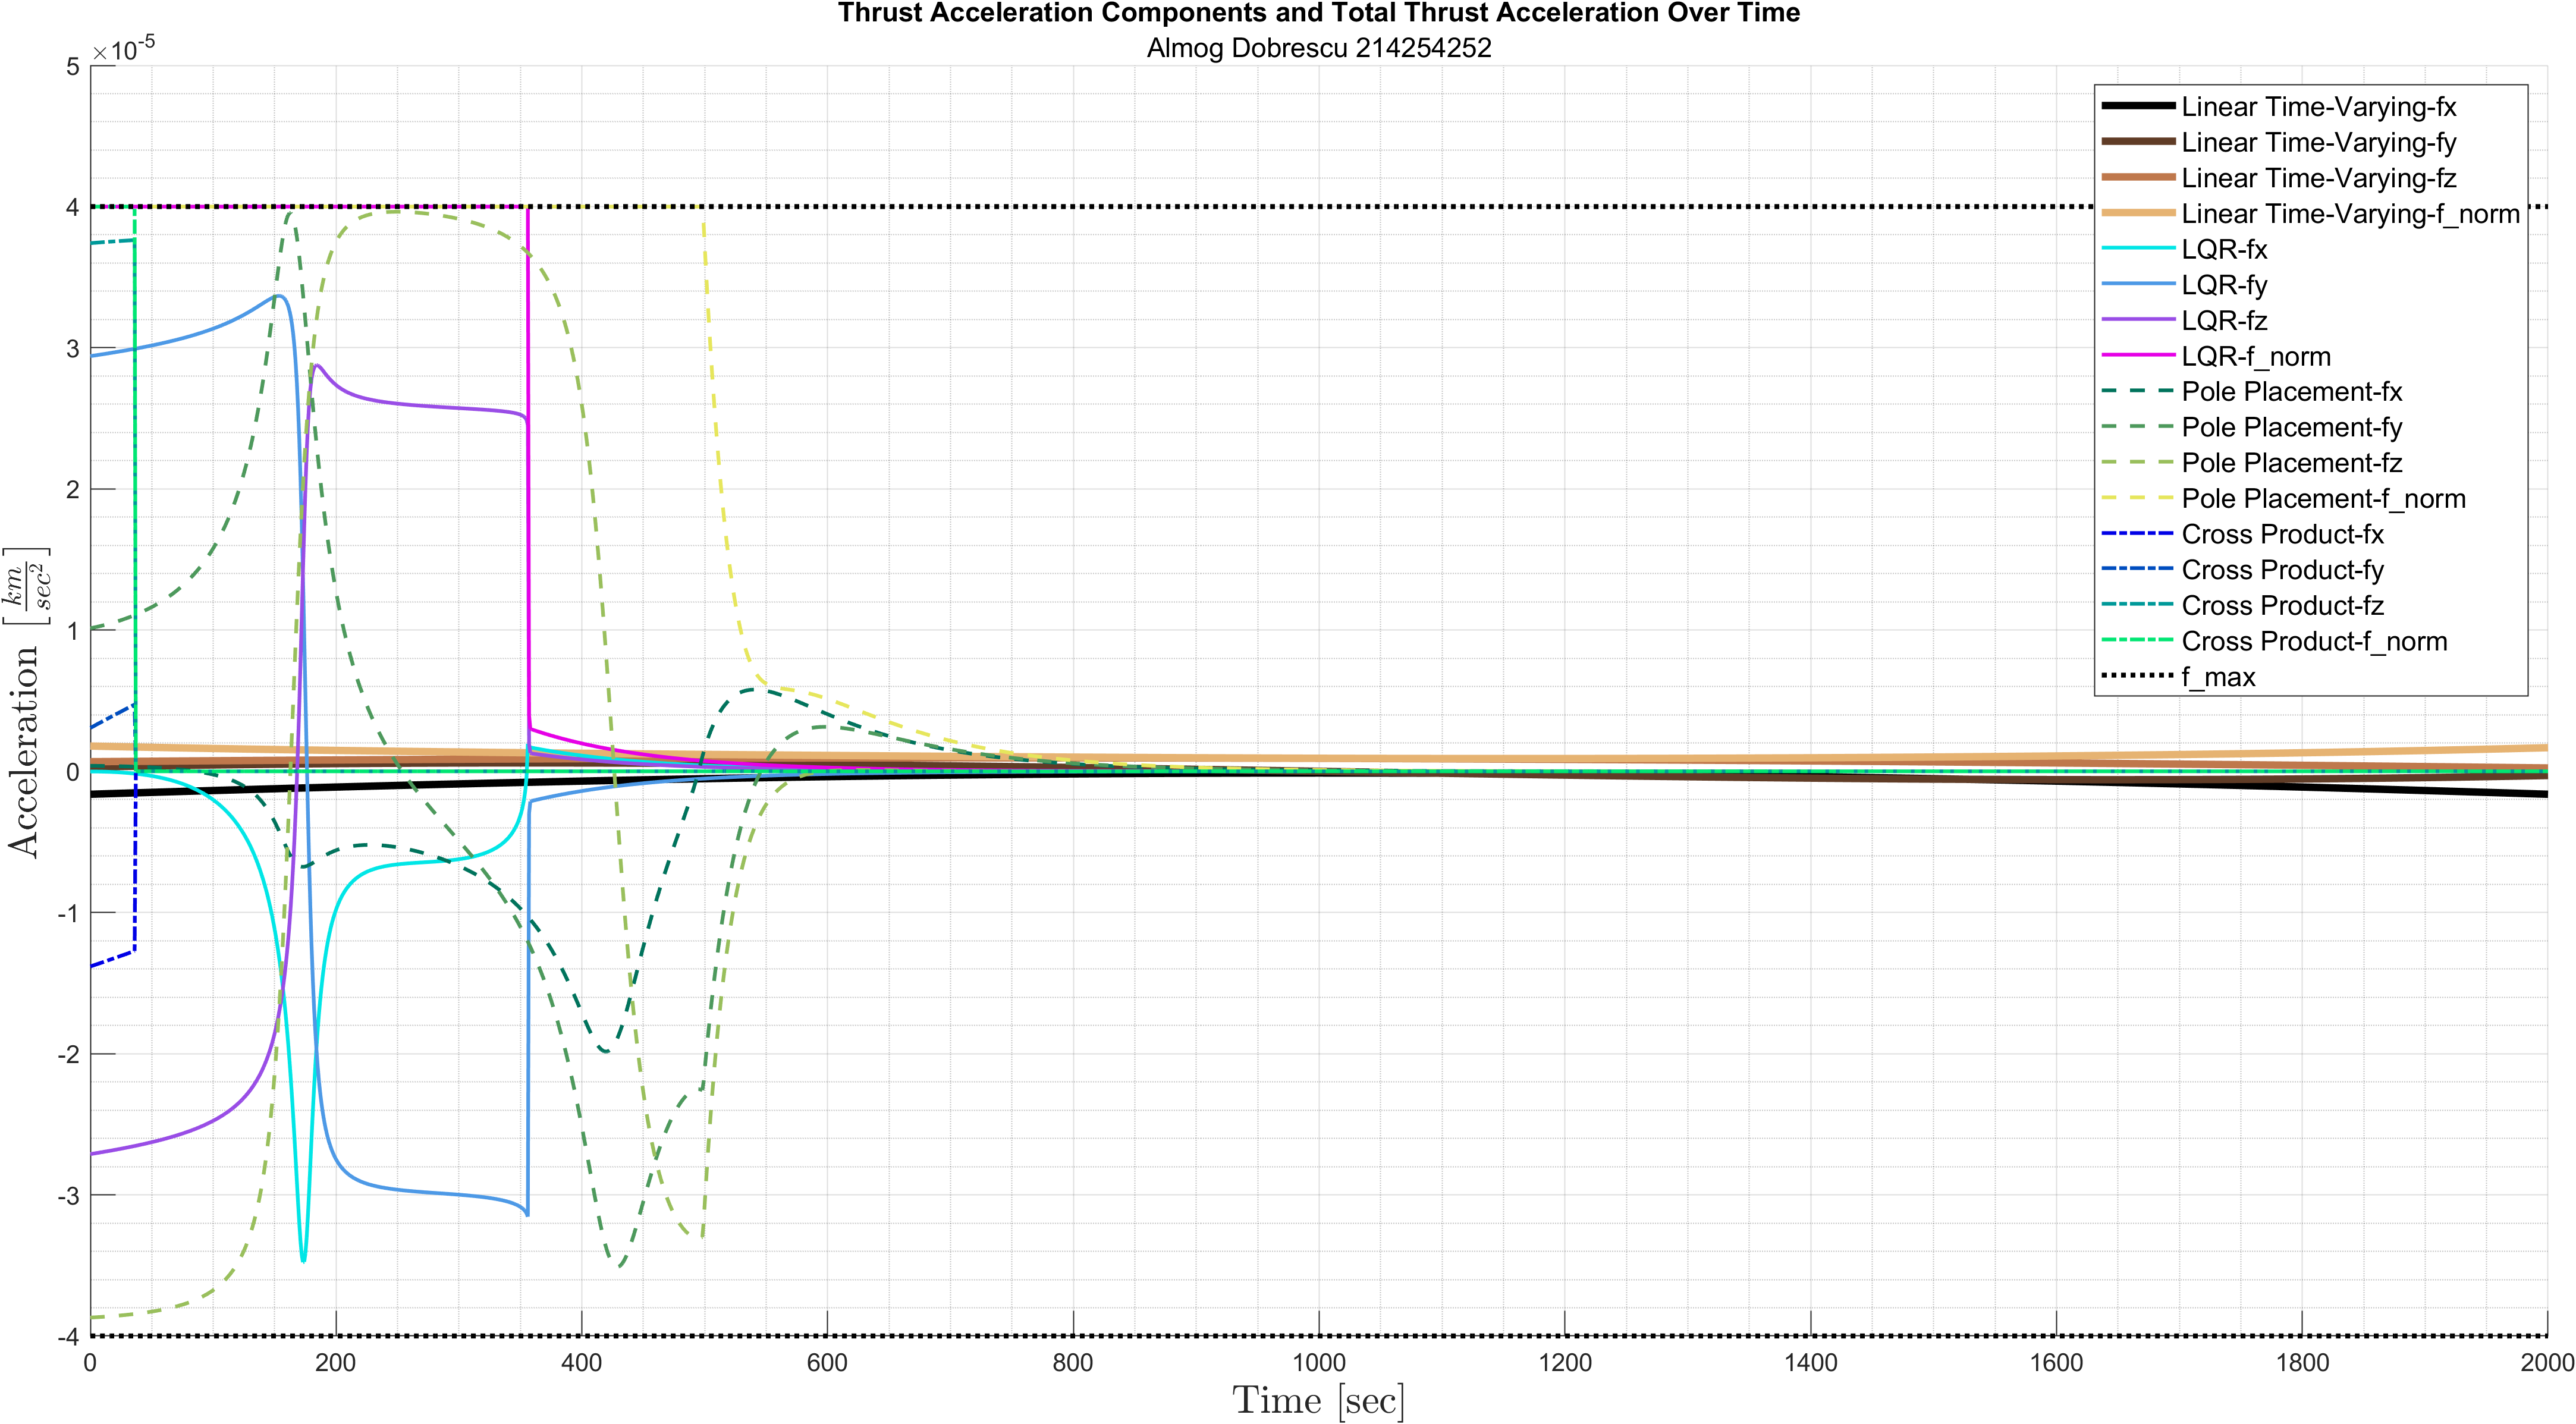
\includegraphics[width=1\textwidth]{images/graph3.png}
    \caption{Thrust acceleration components and total thrust acceleration over time}
    \label{fig:accel_over_time}
\end{figure}
\begin{figure}[H]
    \centering
    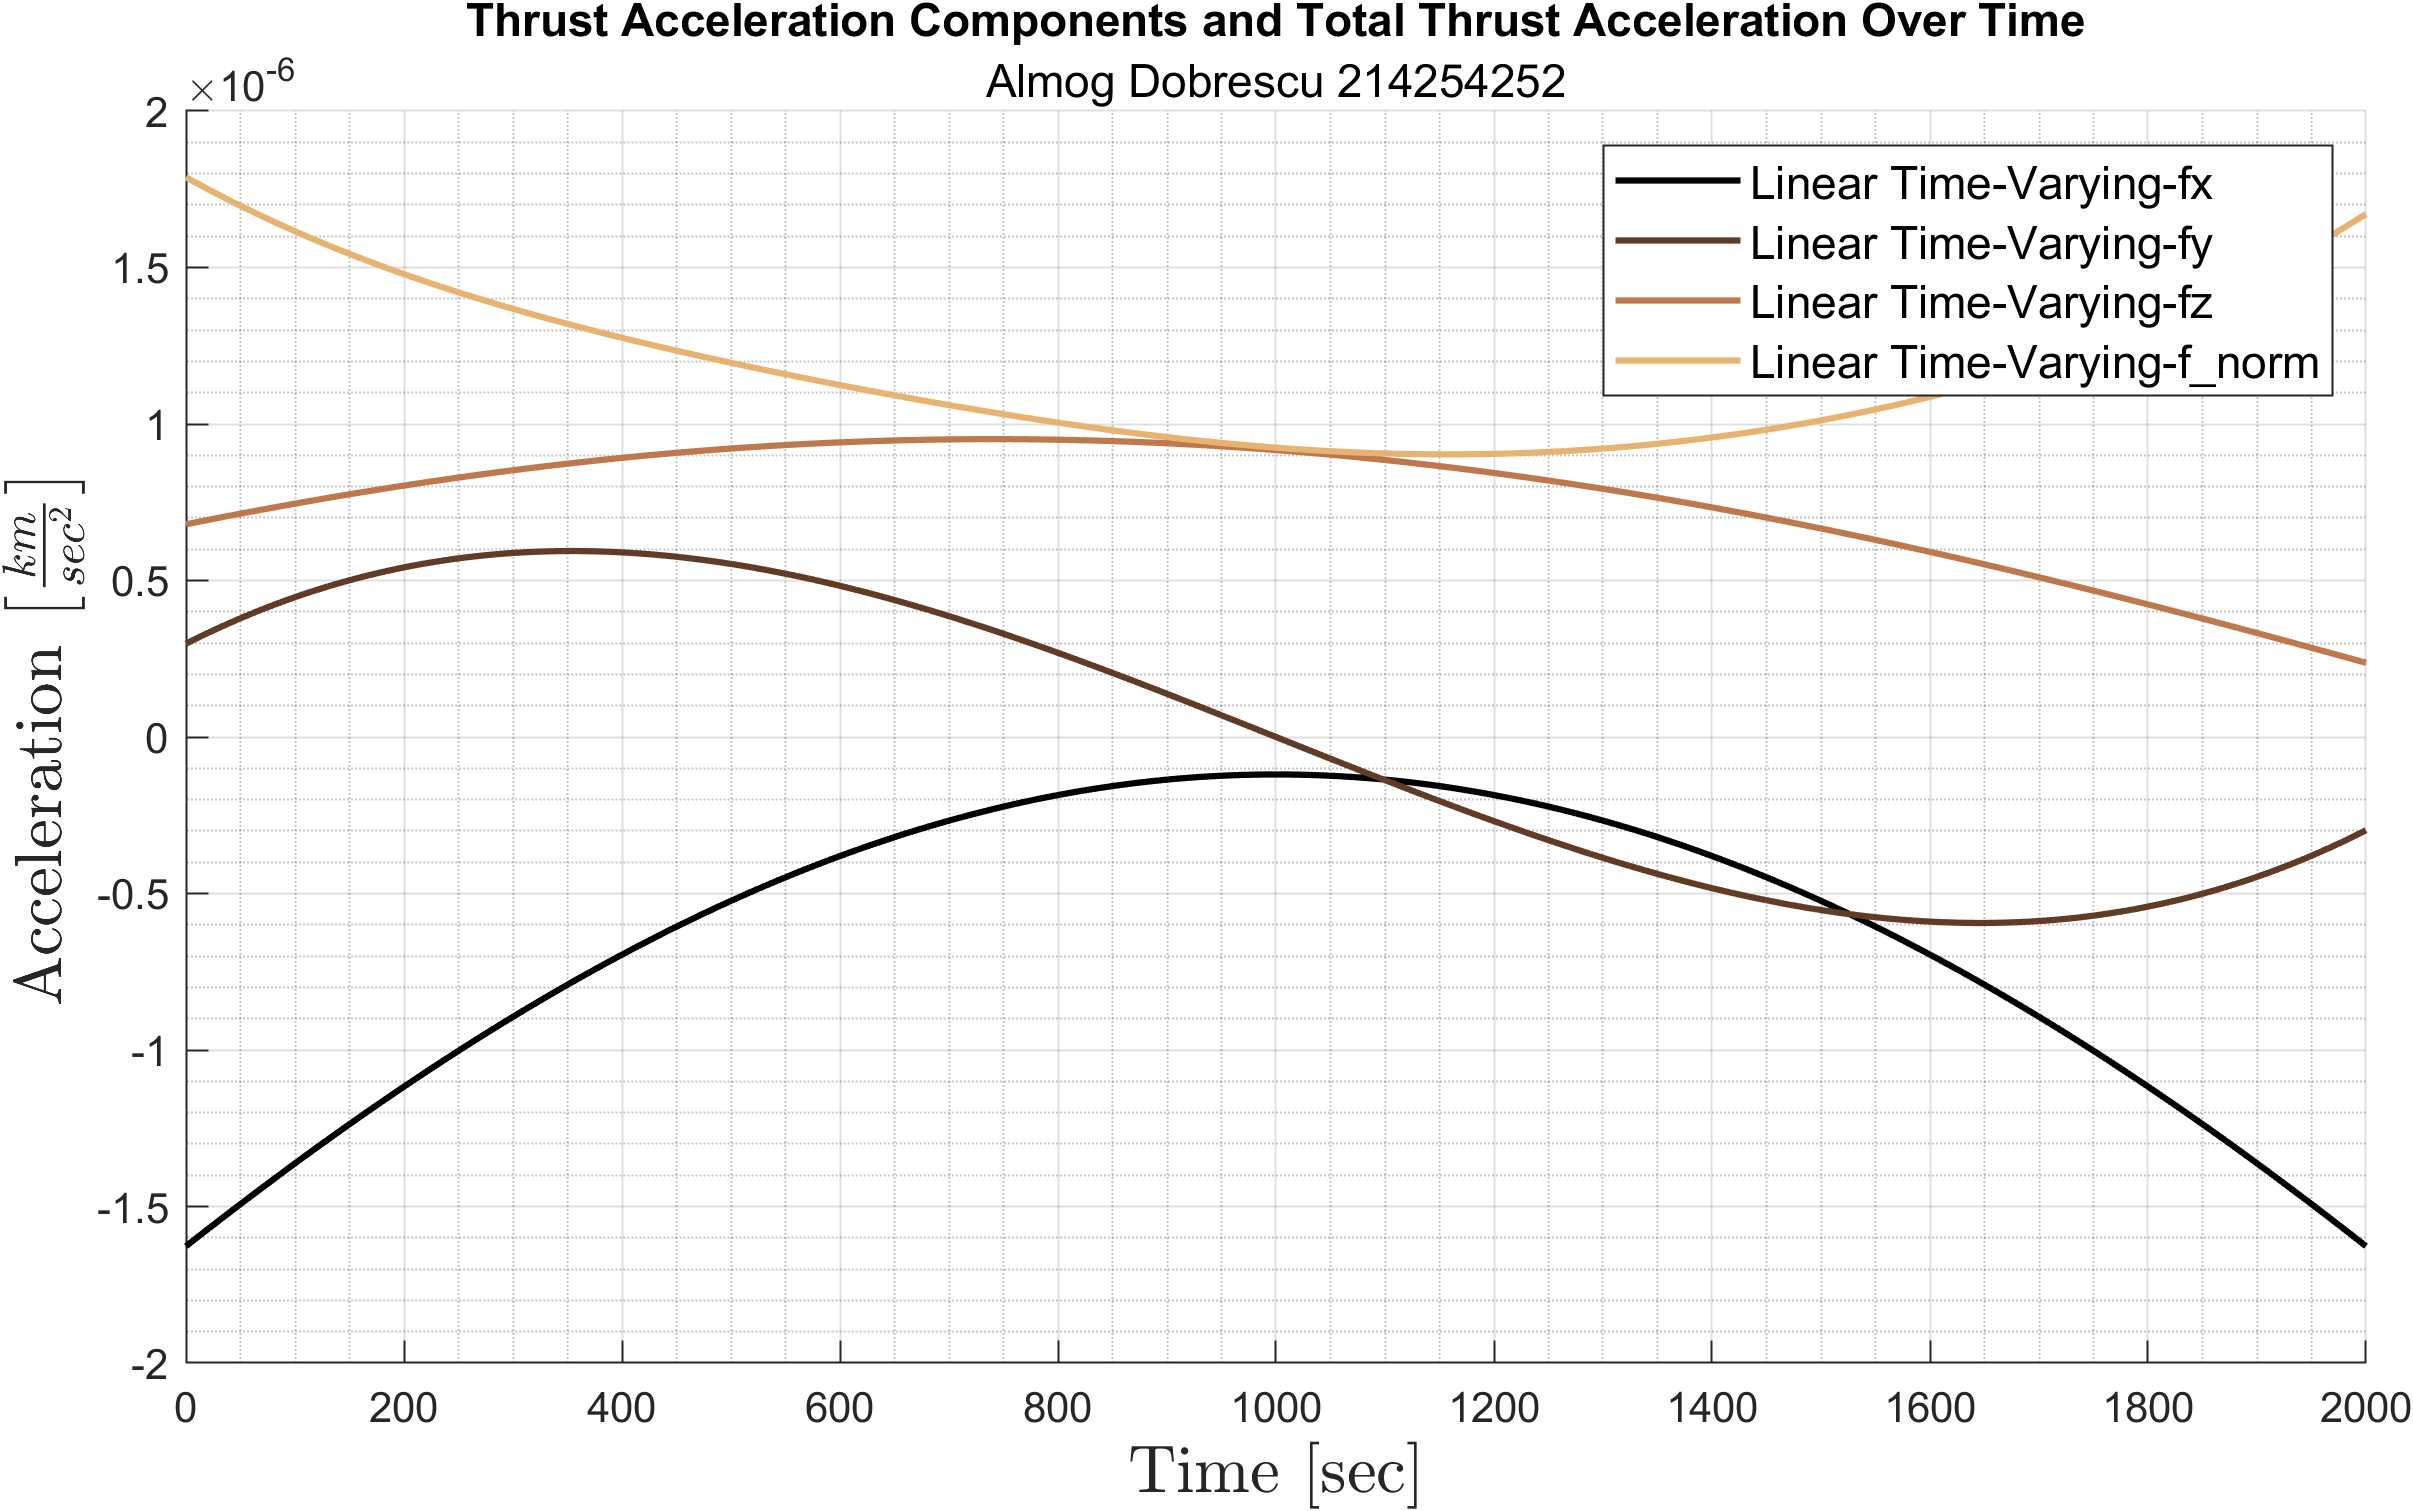
\includegraphics[width=1\textwidth]{images/graph4.png}
    \caption{Thrust acceleration components and total thrust acceleration over time - only HW7}
    \label{fig:accel_over_time_hw7}
\end{figure}
\begin{figure}[H]
    \centering
    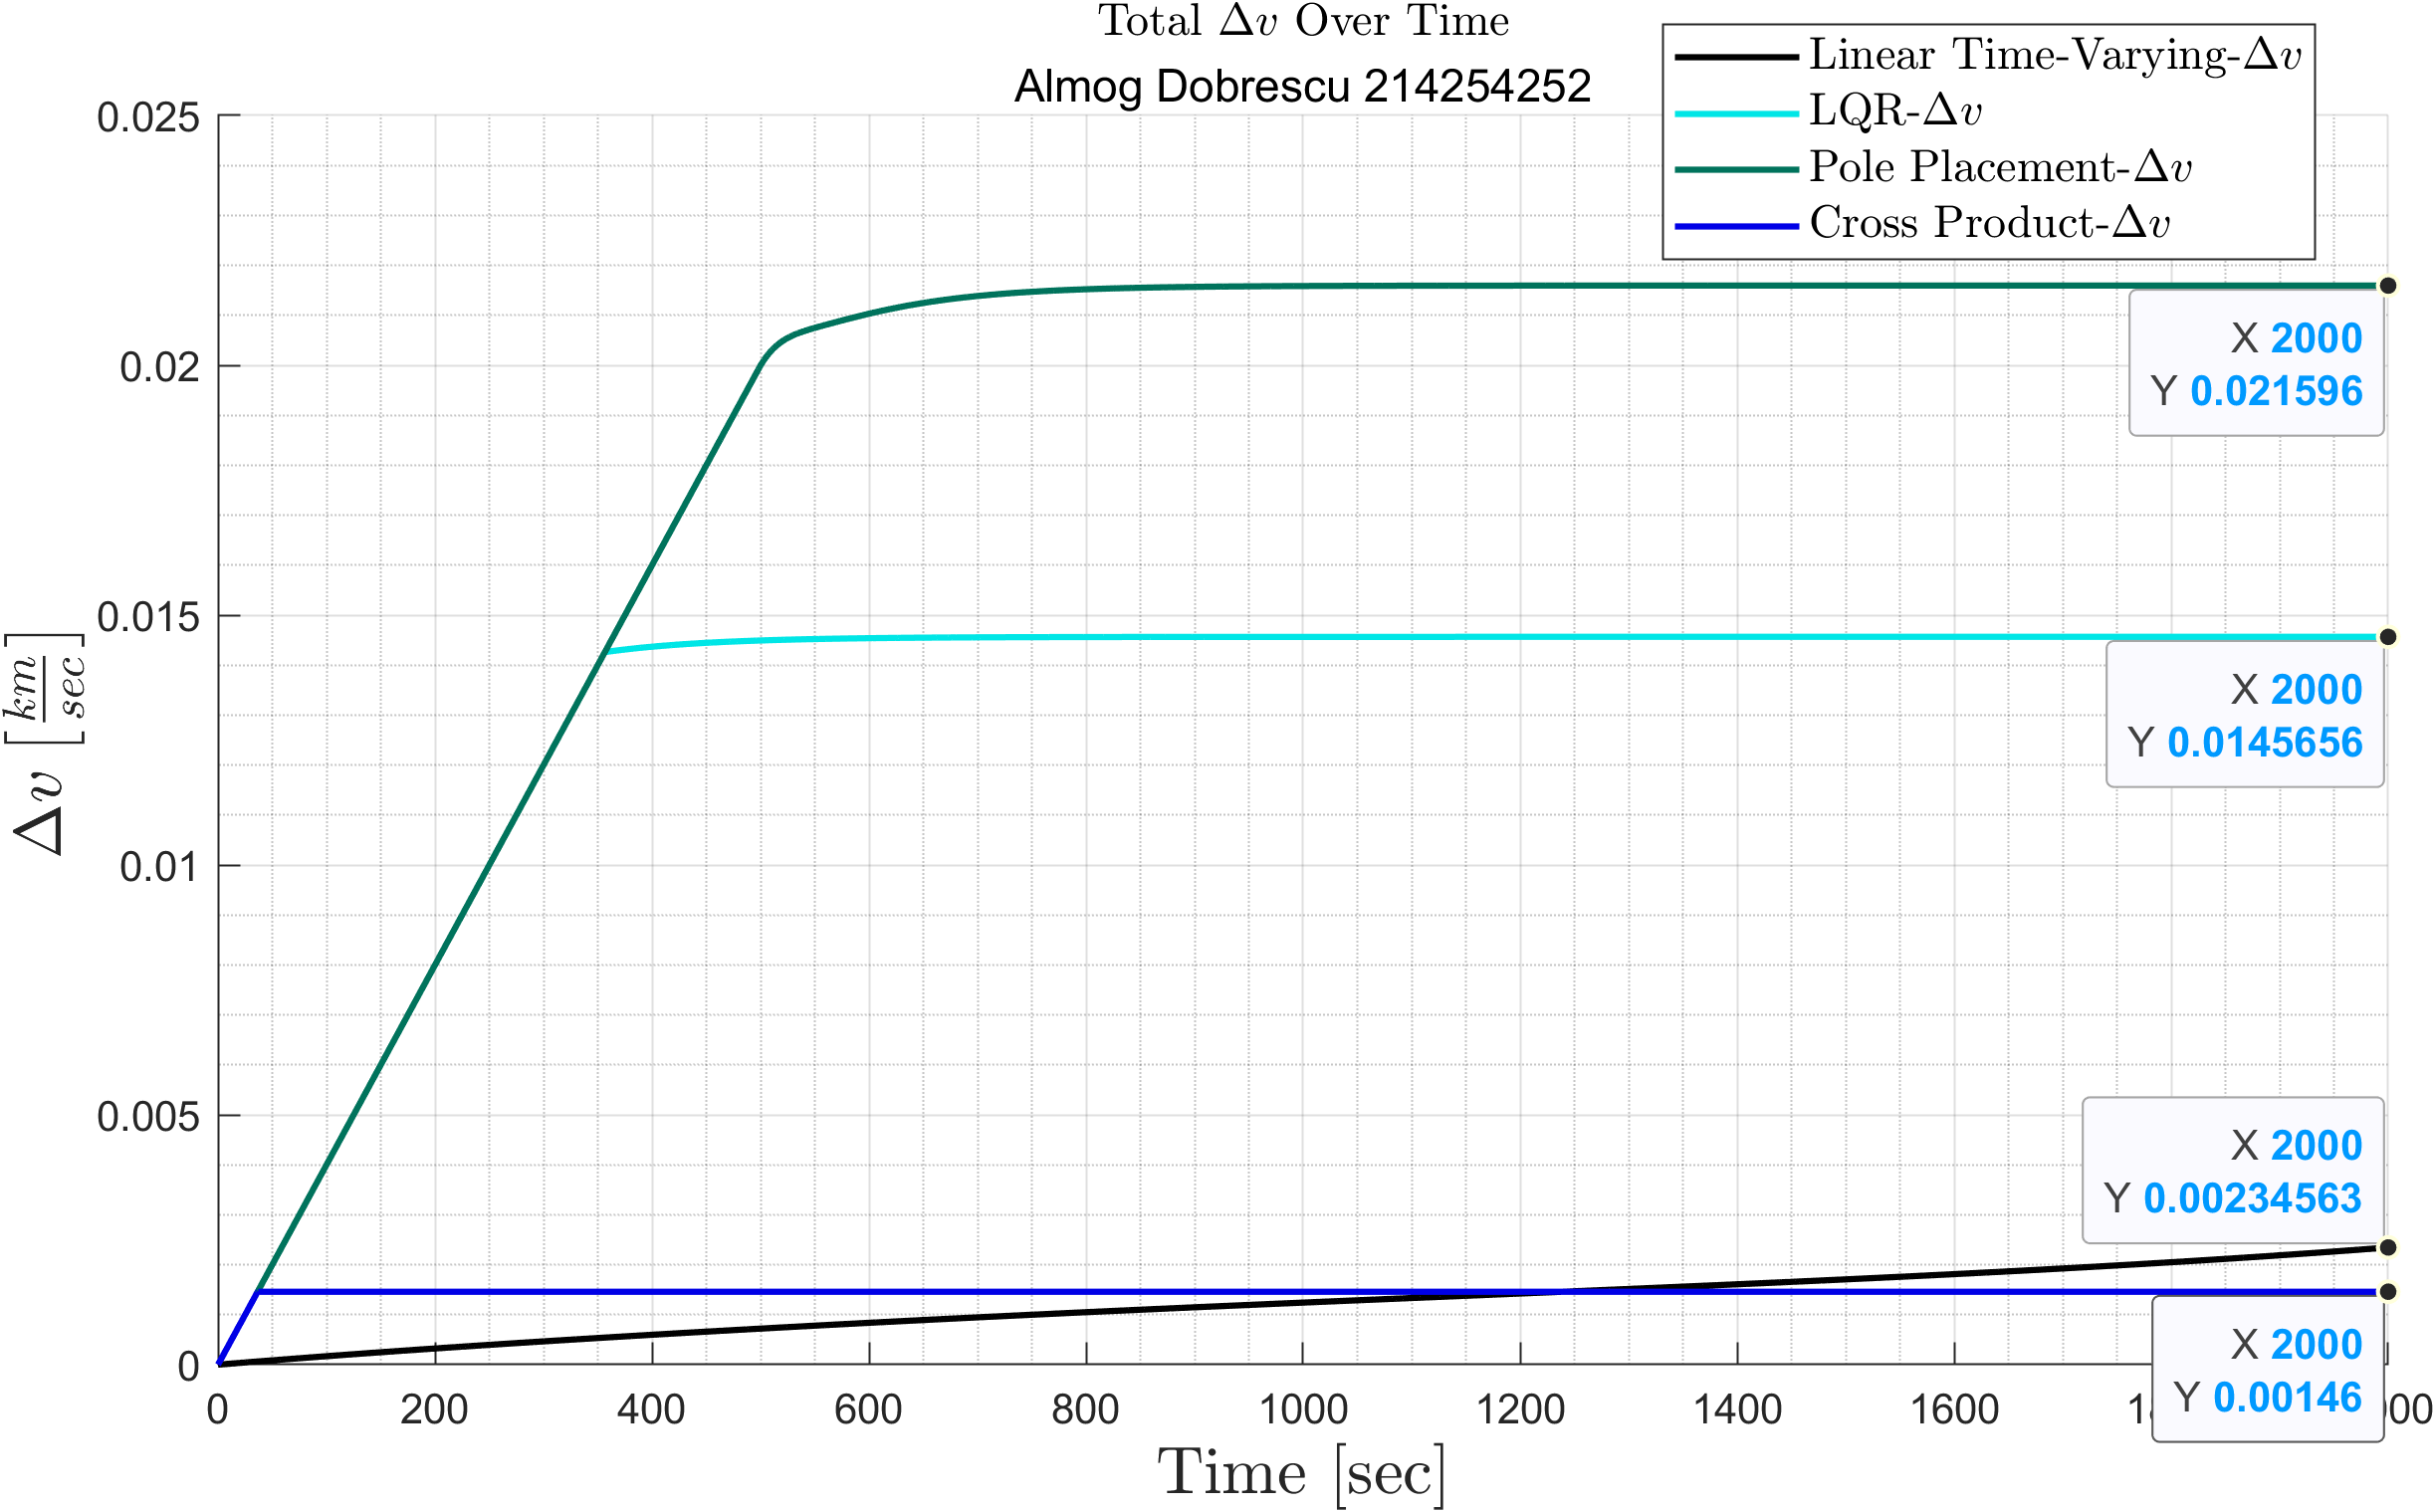
\includegraphics[width=1\textwidth]{images/graph5.png}
    \caption{Total $\Delta v$ over time}
    \label{fig:delta_v_over_time}
\end{figure}
We can see that we indeed acomplished the design criteria:
\begin{itemize}
    \item The thrust doesn't exceed the maximum available thrust.
    \item The miss distance at the final desired time is less than $1[\mathrm{m}]\ \left(7.3649\cdot10^{-12}\left[\mathrm{m}\right]\right)$.
    \item The miss velocity at the final desired time is less than $1\left[\displaystyle\frac{\mathrm{cm}}{\mathrm{sec}}\right]\ \left(1.2791\cdot10^{-12}\left[\displaystyle\frac{\mathrm{cm}}{\mathrm{sec}}\right]\right)$.
\end{itemize}

The total $\Delta v$ is: $0.0023\left[\displaystyle\frac{\mathrm{km}}{\mathrm{sec}}\right]$

\end{document}